\documentclass[polish, twoside, 12pt]{mwart}
\usepackage[polish]{babel}
\usepackage{polski}
\usepackage[T1]{fontenc}
\usepackage[utf8]{inputenc}

\usepackage{hyperref}
\hypersetup{
    colorlinks,
    citecolor=black,
    filecolor=black,
    linkcolor=black,
    urlcolor=black
}
\usepackage{listings}

\usepackage{tikz-qtree}

\usepackage{graphicx}
\graphicspath{ {../figures/} }

\let\stdsection\section
\renewcommand*{\section}{\clearpage\stdsection}
\emergencystretch=3em
\linespread{1.1}

\author{Kewin Polok}
\title{Praca dyplomowa magisterska}

\begin{document}

\maketitle
 
\newpage

\tableofcontents

\newpage

\listoffigures
 
\listoftables

\newpage

\section{Wstęp}

\subsection{Cel pracy}

\subsection{Układ pracy}

\section{Specyfikacja problemu}

\subsection{Założenia dotyczące problemu}

\section{Przeglądarka internetowa}

Przeglądarka internetowa (ang. \emph{web browser}) to program komputerowy służący do pobierania i wyświetlania stron internetowych udostępnianych przez serwery WWW. Komunikacja z serwerem odbywa się najczęściej za pomocą protokołu HTTP (ang. \emph{Hypertext Transfer Protocol})lub odpowiednika w wersji szyfrowanej HTTPS (ang. \emph{Hypertext Transfer Protocol Secure}). Nierzadko przeglądarki internetowe są w stanie obsługiwać inne protokoły takie jak np. FTP (ang. \emph{File Transfer Protocol}) wykorzystywany do serwerów plików, czy też protokoły POP3 (ang. \emph{Post Office Protocol}), IMAP (ang. \emph{Internet Message Access Protocol}) i SMTP (ang. \emph{Simple Mail Transfer Protocol}) wykorzystywane do poczty elektronicznej. 

\begin{figure}[ht]
  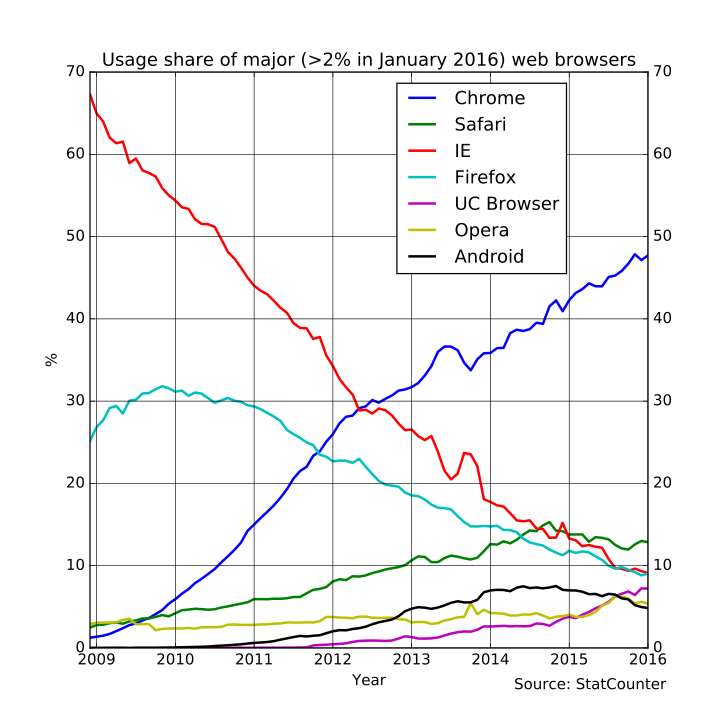
\includegraphics[width=\textwidth]{web-browers-usage-share.png}
	\caption{Udział najwaznieższych przeglądarek na rynku w latach 2009-2016}
\end{figure}

\subsection{Technologie}

Współczesne strony internetowe to nierzadko bardzo skompliowane aplikacje, dlatego też przeglądarki internetowe muszą bardzo dobrze obsługiwać wiele technologii, które działając razem pozwalają dostarczyć bardzo wysokiej jakości doświadczenia użytkownika (ang. \emph{User experience}). 

\subsubsection{HTML 5.1} \label{html}

Hipertekstowy język znaczników (ang. \emph{HyperText Markup Language}) to język służący do określenia struktury strony internetowej. Definicję HTML 5.1 stanowi W3C REC-HTML51 \cite{w3c-rec-html51}. Oprócz głównego tekstu HTML zawiera tak zwane znaczniki, które zawierają dodatkowe informacje pozwalające przeglądarce internetowej odpowiednio zinterpretować określony fragment strony interetowej. Za pomocą znaczników możemy formować fragmenty strony w takie struktury jak hiperłącza, akapity, listy, nagłówki, czy też formularze. Znaczniki najczęściej występują w parach (jako znacznik otwierając oraz zamykający) definiując zakres działania.

\lstinputlisting[language=HTML, caption=Przykładowa prosta strona internetowa z formularzem]{../src/examples/html.html}

Strona internetowa zaczyna się od \emph{<!DOCTYPE html>}. Jest to specjalny znacznik, który musi być umieszczony jako pierwszy. Informuje on przeglądarkę o tym, że tekst jest w formacie HTML. Kolejnym znacznikiem jest \emph{html} z atrybutem \emph{lang}, jest to główny znacznik, będacy korzeniem całej zagnieżdzonej struktury. Dodatkowo informuje o. Bardzo ważny, wyraźnie odseparowany fragment to znacznik \emph{head} zawierający infomację o systemie kodowania (w tym wypadku jest to  kodowanie UTF-8) oraz tytuł strony. Może on zawierać dodatkowe metadane opisujące stronę internetową. Z punktu widzenia użytkownika najważniejszym fragmentem jest znacznik \emph{body}, który zawiera właściwą treść, czyli w tym wypadku jest to głównie formularz \emph{form}. Dwa najważniejsze atrybuty opisujące formularz to \emph{action} informujący przeglądarkę gdzie wysłać dane wpisane przez użytkownika oraz \emph{method} na podstawie, którego przeglądarka wie jaką metodę protokołu HTTP zastosować. Przykładowy formularz zawiera jedno pole tekstowe \emph{input type="text"} oraz jedno pole do wpisywania haseł \emph{input type="password"}. Hasło wpisane w tego typu pole jest domyślnie ukryte przez przeglądarkę dla celów bezpieczeństwa. Oba pola dodatkowo opisane są etykietami \emph{label}. Ostatnim nieopisanym jeszcze znacznikiem jest \emph{button type="submit"}, który jest po prostu przyciskiem służącym do wysłania formularza. Każda przeglądarka posiada wbudowany zestaw styli, który definiuje wygląd każdego znacznika przewidzianego w dokumentacji HTML 5.

\begin{figure}[ht]
  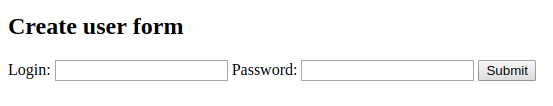
\includegraphics[width=\textwidth]{html-chrome.png}
	\caption{Przykład wyrenderowany w przeglądarce Chrome}
\end{figure}

\subsubsection{CSS 3}

Kaskadowe arkusze stylów (ang. \emph{Cascading Style Sheets}) to język służący do opisu wyświetlania struktury opisanej w języku HTML. Wersja 3 składa się z wielu modułów. Każdy z nich dodaje nowe możliwości lub rozszerza te zdefiniowane w CSS 2 zachowując wsteczną kompatybilność (ang. \emph{backward compatibility}).

\begin{enumerate}
  \item css3-background - specyfikacja W3C REC-CSS3-Background \cite{w3c-rec-css3-background}
  \item css3-box - specyfikacja W3C REC-CSS3-Box \cite{w3c-rec-css3-box}
  \item css-cascade-3 - specyfikacja W3C REC-CSS-Cascade-3 \cite{w3c-rec-css3-cascade}
  \item css3-color - specyfikacja W3C REC-CSS3-Color \cite{w3c-rec-css3-color}
  \item css3-content - specyfikacja W3C REC-CSS-Content-3 \cite{w3c-rec-css3-content}
  \item css-fonts-3 - specyfikacja W3C REC-CSS-Fonts-3 \cite{w3c-rec-css3-fonts}
  \item css3-gcpm - specyfikacja W3C REC-CSS-GCPM-3 \cite{w3c-rec-css3-gcpm}
  \item css3-layout - specyfikacja W3C REC-CSS-Template-3 \cite{w3c-rec-css3-template}
  \item css3-mediaqueries - specyfikacja W3C REC-CSS3-Mediaqueries \cite{w3c-rec-css3-mediaqueries}
  \item css3-multicol - specyfikacja W3C REC-CSS3-Multicol \cite{w3c-rec-css3-multicol}
  \item css3-page - specyfikacja W3C REC-CSS3-Page \cite{w3c-rec-css3-page}
  \item css3-selectors - specyfikacja W3C REC-CSS3-Selectors \cite{w3c-rec-css3-selectors}
  \item css-3-ui - W3C REC-CSS-UI-3 \cite{w3c-rec-css3-ui}
\end{enumerate}

Za pomocą CSS opisać można wszystkie pojęcia odpowiedzialne za reprezentację elementów HTML, takie jak rodzina czcionek, kolor tekstu, marginesy, czy też pozycja danego elementu względem innych elementów lub okna przeglądarki.

CSS został stworzony w celu odseparowania struktury dokumentu od formy jego prezentacji. Zalety tej separacji to zwiększony zakres dostępności witryny, zmniejszona zawiłość dokumentu, łatwiejsze wprowadzanie zmian w strukturze dokumentu. CSS ułatwia także zmiany w wyświetlaniu strony w zależności od obsługiwanego medium (ekran komputera, ekran tabletu, ekran telefonu komórkowego).

Arkusz stylów składa się z reguł określających styl dla wybranych elementów dokumentu. Reguła składa się z selektora oraz deklaracji. Selektor określa grupę elementów, którego ma dotyczyć deklaracja. Deklaracja określa formatowanie i składa się z nazwy jednej z właściwości i jej wartości napisanej po dwukropku. Deklaracja musi być otoczona nawiasami klamrowymi.

\begin{lstlisting}
selektor { 
	wlasciwosc: wartosc; 
}
\end{lstlisting}

Selektory oraz deklaracje można grupować. Zgrupowane selektory rozdziela się przecinkami, natomiast deklaracje średnikami.

\begin{lstlisting}
selektor, selektor2 { 
	wlasciwosc1: wartosc1;
	wlasciwosc2: wartosc2;
}
\end{lstlisting}

Selektory mogą poszukiwać elementy na podstawie wielu różnych wartośći, jedne z nich to:

\begin{itemize}
  \item nazwa elementu np. \emph{h1}
  \item atrybut \emph{class} elementu np. \emph{.my-class}
  \item identyfikator elementu, czyli atrybut \emph{id} np. \emph{\#element-id}
  \item połączenie wcześniejszych selektorów operatorem logicznym \emph{OR} np. \emph{h1.my-class}
  \item połączenie wcześniejszych selektorów operatorem logicznym \emph{AND} np. \emph{\#element-id .my-class}
\end{itemize}

Dobrą praktyką jest definiowanie selektorów na podstawie atrubutu \emph{class}, natomiast identyfikator, czyli atrybut \emph{id} powinien służyć do jednoznacznej identyfikacji elementu w strukturze HTML. Zgodnie z dokumentacją wiele znaczników może posiadać taką samą klasę, natomiast identyfikator aby spełniał swoje zadanie musi być unikalny.

Ponieważ standardowy wygląd znaczników z punktu widzenia użytkownika może być interpretowany jako bardzo prosty to współcześnie nieostylowane strony internetowe zdarzają się bardzo rzadko. W celu pokazania jak duża może być różnica pomiędzy standardowym, a specjalnie ostylowanym wyglądem strony internetowej przedstawiony zostanie poprzedni przykład strony z formularzem wzbogacony o bardzo lekką bibliotekę CSS o nazwie Milligram\cite{milligram}, której rozmiar wynosi tylko 2kb.

\begin{figure}[ht]
  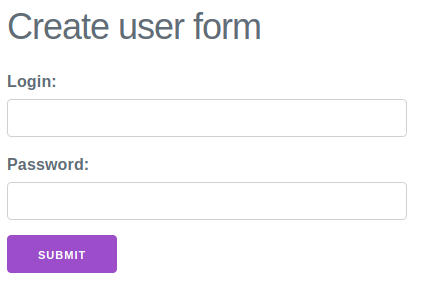
\includegraphics[width=\textwidth]{html-css-chrome.png}
	\caption{Ostylowany przykład wyrenderowany w przeglądarce Chrome}
\end{figure}

\subsubsection{JavaScript}

JavaScript to skryptowy język programowania, stworzony przez firmę Netscape, najczęściej stosowany na stronach internetowych. Pod koniec lat 90. XX wieku organizacja ECMA wydała na podstawie JavaScriptu standard języka skryptowego o nazwie ECMAScript. Najnowsza stabilna wersja ECMAScript nosi nazwę ECMAScript 2016 \cite{es2016} i została wydana 17 czerwca 2016. Organizacja ECMA zapowiedziała, że stabilna wersja tego standardu od wersji 2015 będzie ogłaszana co rok i to właśnie rok wydania będzie jednoznaczny z numerem wersji. Wcześniej mowa była o edycji standardu ECMAScript i do teraz często można się spotkać z zamiennem stosowaniem nazw ECMAScript 6 i ECMAScript 2015 (skracanych odpowiednio do ES6 i ES2015).

Najczęściej spotykanym zastosowaniem języka JavaScript są strony WWW. Skrypty napisane w tym języku najczęściej służą do zapewnienia interaktywności poprzez odpowiednie reagowanie na zdarzenia generowane przez użytkownika. Skrypty JavaScriptu uruchamiane przez strony internetowe mają znacznie ograniczony dostęp do komputera użytkownika. 

Platformy programistyczne, które zostaną zbadane w ramach pracy magisterskiej napisane są języku JavaScript. Wspomagają one proces pisania aplikacji internetowej dostarczając odpowiednich funkcji i organizująć strukturę strony internetowej zgodnie z wytycznymi konkretnej platformy programistycznej.

W języku HTML za umieszczanie skryptów JavaScript odpowiedzialny jest znacznik \emph{script} z opcjonalnymi parametrami \emph{type="text/javascript"} i \emph{language="javascript"}.

JavaScript może zostać użyty również po stronie serwera dzięki darmowemu środowisku uruchomieniowemu Node.js\cite{node.js}. Node.js zaprojektowany został do tworzenia wysoce skalowalnych aplikacji internetowych, szczególnie właśnie serwerów napisanych w języku JavaScript. Architektura Node.js składa się z silnika V8 \cite{v8} stworzonego przez Google i opiera się na sterowaniu zdarzeniami wykorzystującymi asynchroniczny system wejścia-wyjścia. Kod źródłowy jest otwarty (ang. \emph{open source}) i każdy może brać udział w jego rozwijaniu. Domyślnym menedżer pakietów dla Node.js jest Npm \cite{npm}, jednak warto zapoznać się z alternatywnym mendedżerem o nazwie Yarn \cite{yarn}, którego głównymi zaletami są szybsze pobieranie zależności oraz bardziej płaska stuktura drzewa pobranych zależności.

\subsubsection{DOM} \label{dom}

Obiektowy model dokumentu (ang. \emph{Document Object Model}) to zespół klas i interfejsów programistycznych umożliwiających dostęp do elementów strony napisanej w języku HTML. Istnieje kilka tzw. poziomów DOM (ang. \emph{level}):

\begin{enumerate}
  \item DOM Level 0 - nie stanowi oficjalnego standardu W3C \cite{w3c}, pierwotnie był modelem zaimplementowanym w przeglądarce Netscape Navigator 3.0, obecnie wspierają go wszystkie przeglądarki
  \item DOM Level 1 - specyfikacja W3C REC-DOM-Level-1 \cite{w3c-rec-dom-level-1} 
  \item DOM Level 2 - specyfikacja W3C REC-DOM-Level-2 \cite{w3c-rec-dom-level-2} 
  \item DOM Level 3 - definicję stanowi sześć specyfikacji
  \begin{itemize}
    \item DOM Level 3 Core - specyfikacja W3C DOM-Level-3-Core \cite{w3c-rec-dom-level-3-core}
    \item DOM Level 3 Load and Save - specyfikacja W3C DOM-Level-3-LS \cite{w3c-rec-dom-level-3-ls}
    \item DOM Level 3 XPath - specyfikacja W3C DOM-Level-3-XPath \cite{w3c-rec-dom-level-3-xpath}
    \item DOM Level 3 Views and Formatting - specyfikacja W3C DOM-Level-3-Views \cite{w3c-rec-dom-level-3-views}
    \item DOM Level 3 Requirements - specyfikacja W3C DOM-Level-3-Requirements \cite{w3c-rec-dom-level-3-requirements}
    \item DOM Level 3 Validation - specyfikacja W3C DOM-Level-3-Val \cite{w3c-rec-dom-level-3-val}
  \end{itemize}
\end{enumerate}

DOM pozwala dokonywać dowolnych modyfikacji poprzez tworzenie, usuwanie i modyfikację tzw. węzłów (ang. \emph{nodes}). Początkowo nie istniał standardowy obiektowy model dokumentu. Twórcy najpopulaniejszych przeglądarek tworzyłi własne niezgodne ze sobą modele. Organizacja W3C \cite{w3c} przygotowała ujednolicony standard obiektowego modelu dokumentu, w którym dokment jest dostępny pod postacią globalnego obiektu \emph{document}, który posiada metody do np. pobierania elementu na podstawie identyfikatora \emph{document.getElementById} lub na podstawie klasy \emph{document.getElementByClassName}. Standard W3C definiuje interfejsy DOM tylko dla języków JavaScript i Java.

\begin{figure}
  \centering
  \begin{tikzpicture}
    \Tree[.html 
      [.head 
        [.meta ]
        [.title ]
      ]
      [.body 
        [.h2 ]
        [.form 
            [.label ]
            [.input ]
            [.label ]
            [.input ]
            [.button ]
        ]
      ]
    ]
  \end{tikzpicture}
  \caption{Drzewo DOM wygenerowane dla przykładu opisanego w rozdziale \ref{html}}
\end{figure}

\subsubsection{CSSOM} \label{cssom}

Obiektowy model kaskadowych arkuszy stylów (ang. \emph{CSS Object Model}) to zespoł interfejsów programistycznych umożliwiających dostęp do stylów napisanych w języku CSS.

CSSOM blokuje wszystko przed wyświetleniem tzn. przeglądarka internetowa nie zacznie niczego renderować dopóki w pełni nie zostanie zakończona budowa CSSOM. W przypadku nieoptymalnej struktury CSS budowa może trwać bardzo długo co skutkuje widoczną dla użytkownika białą stroną bez zawartości.

CSSOM musi być zbudowany na nowo z każdym przeładowaniem strony, oznacza to, iż nawet jeśli pliki CSS zostały umieszczone w pamięci podręcznej (ang. \emph{cache}) to nie uchroni to przeglądarki przed koniecznością budowy CSSOM.

Istnieje związek pomiędzy kaskadowymi arkuszami stylów, które przeglądarka ładuje i skryptami JavaScript umieszczonymi na stronie. Żeby przeglądarka wyświetliła cokolwiek musi poprawnie zakończyć budowę CSSOM, w przypadku gdy budowa ta zostanie wstrzymana przez skrypty czas potrzebny na wyświetlenie jakiegokolwiek elementu wzrośnie. W przypadku nieoptymalnej kombinacji skryptów oraz stylów czas ten może wzrosnąc drastycznie skutkując bardzo negatywnymi doświadczeniami użytkownika, w najgorszym wypadku spowodować zniechęcenie użytkownika do dalszego oczekiwania i opuszczenie strony.

\begin{figure}
  \centering
  \begin{tikzpicture}
    \Tree[.body(font-size:10px) 
      [.h1(font-size:1.6rem) ]
      [.form(font-size:1.4rem) 
        [.label(font-size:1.2rem) ]
        [.input(font-size:1.2rem) ]
      ]
      [.button(font-size:1.4rem) ]
    ]
  \end{tikzpicture}
  \caption{Przykładowe drzewo CSSOM wygenerowane dla przykładu opisanego w rozdziale \ref{html}}
\end{figure}

\subsubsection{HTTP/1.1} \label{http/1.1}

Protokół przesyłania dokumentów hipertekstowych (ang.\emph{(Hypertext Transfer Protocol)}) to protokół za pomocą którego przysła się żadania udostępnienia dokumentów z serwera WWW oraz informacje z forumlarzy internetowych. Obecną definicję HTTP stanowi RFC 2616 \cite{rfc2616}

Protokół HTTP udostępnia znormalizowany sposób komunikowania się komputerów ze sobą. Określa on formę żądań (ang. \emph{requests}) klienta dotyczących danych oraz formę odpowiedzi (ang. \emph{responses}) serwera na te żądania. Klientem może być np. przeglądarka internetowa. Jest zaliczany do protokołów bezstanowych (ang. \emph{stateless}) ponieważ nie zachowuje żadnych informacji o poprzednich transakcjach z klientem. Pozwala to znacznie zmniejszyć obciążenie serwera, jednak uniemożliwia zapamiętanie konkretnego stanu użytkownika w sytuacji gdy jest to potrzbne np. przy implementacji koszyka z zakupami w sklepie internetowym. Najczęstszym rozwiązaniem tego problemu jest wprowadzenie mechanizmu ciasteczek (ang. \emph{cookies}). Ciasteczka to mały fragment tekstu zawierający pary klucz-wartość. Przesyłane są one z każdym żądaniem do serwera. Alternatywne rozwiązania to ukryte parametry (gdy aktualna strona zawiera formularz) oraz parametry umieszczone w ujednoliconym formacie adresowania zasobów (ang. \emph{Uniform Resource Locator}.

Wywołania protokołu HTTP zaczynają się od \url{http://}. HTTP standardowo korzysta z portu numer 80 protokołu kontroli transmisji (ang. \emph{Transmission Control Protocol}).

Zapytanie HTTP zaczynaja się od nazwy metody, która określa akcję jaką obiekt tworzący zapytanie chce wykonać na zasobie podstępnym pod określonym adresem. Dostępne metody to:

\begin{enumerate}
  \item \emph{GET} - pobranie zasobu
  \item \emph{HEAD} - pobranie informacji o zasobie, metoda stosowana do sprawdzania dostępności zasobu
  \item \emph{PUT} - aktualizacja zasobu
  \item \emph{POST} - stworzenie nowego zasobu
  \item \emph{DELETE} - usunięcie zasobu
  \item \emph{OPTIONS} - pobranie informacji o możliwych operacjach do wykonania na zasobie
  \item \emph{TRACE} - metoda stosowana do diagnostyki kanału komunikacyjnego
  \item \emph{PATCH} - częściowa aktualizacja zasobu
\end{enumerate}

Poniżej przedstawione przykładowe żądanie HTTP/1.1 przeglądarki Chrome i odpowiedź serwera opisanego w rozdziale \ref{server}.

\begin{lstlisting}[caption=Przykładowe żądanie HTTP/1.1,]
GET / HTTP/1.1
Host: localhost:8080
Connection: keep-alive
Pragma: no-cache
Cache-Control: no-cache
Upgrade-Insecure-Requests: 1
User-Agent: Mozilla/5.0 (X11; Linux x86_64) AppleWebKit/537.36 
  (KHTML, like Gecko) Chrome/60.0.3112.90 Safari/537.36
Accept: text/html,application/xhtml+xml,application/xml;q=0.9,
  image/webp,image/apng,*/*;q=0.8
Accept-Encoding: gzip, deflate, br
Accept-Language: pl-PL,pl;q=0.8,en-US;q=0.6,en;q=0.4
\end{lstlisting}

\begin{lstlisting}[caption=Przykładowa odpowiedź HTTP/1.1]
HTTP/1.1 200 OK
X-Powered-By: Express
Content-Type: text/html; charset=utf-8
Content-Length: 116
ETag: W/"74-IGpXmXtcB0E/yn+QbK3UFXMrMU8"
Date: Tue, 15 Aug 2017 10:28:41 GMT
Connection: keep-alive
\end{lstlisting}

\subsubsection{HTTPS} \label{https}

Bezpieczny protokół przesyłania dokumentów hipertekstowych (ang. \emph{Hypertext Transfer Protocol Secure}) to szyfrowana wersja protokołu HTTP. Obecną definicję HTTPS stanowi RFC 2660 \cite{rfc2660}

W odróżnieniu od protokołu HTTPS protokół HTTP do komunikacji stosuje niezaszyfrowany tekst. HTTPS początkowo szyfrował dane za pomocą protokołu SSL (ang. \emph{Secure Socket Layer}), natomiast obecnie używany jest protokół TLS (ang. \emph{Transport Layer Security}). Szyfrowanie zapobiega przechtywywaniu i zmienianiu przesyłanych danych. 

Wywołania protokołu HTTPS zaczynają się od \url{https://}. HTTPS standardowo korzysta z portu numer 443 protokołu kontroli transmisji. 

\subsubsection{HTTP/2} \label{http/2}

Protokół HTTP/2 to unowocześniejszego protokołu HTTP/1.1. Został on opracowany na podstawie wczesnych wersji ekperymentalnego protokołu SPDY \cite{spdy}. Obecną definicję HTTP/2 stanowi RFC 7540 \cite{rfc7540}. W przeciwieństwie do wersji HTTP/1.1, protokół HTTP/2 jest w pełni binarny tzn. że tekst zrozumiały dla człowieka zastąpiony został zbiorem tak zwanych ramek (ang. \emph{frames}) o ściśle określonym formacie i zastosowaniu. Poniżej przedstawiono najważniejsze zalety protokołu HTTP/2.

\begin{enumerate}
  \item \emph{Multipleksowanie} - protokół nawiązuje tylko jedno trwałe połączenie z serwerem za pomocą którego pobierane są wszystkie pliku niezbędne do prawidłowego wyświetlenia strony
  \item \emph{Powiadomienia Push} - serwer może wysłać dodatkowe informacje np. może wysłać pliki, które są potrzebne do prawidłowego wyświetlenia strony zanim przeglądarka internetowa zauważy tą potrzebę
  \item \emph{Ustalanie priorytetów} - każde zapytanie o plik posiada swój priorytet, który nadawany jest przez serwer. Umożliwia to najpierw pobranie najważniejszych plików, które pozwolą wyrenderować kluczowe fragmenty strony internetowej, a następnie doczytać kolejne elementy
  \item \emph{Kompresja nagłówków} - protokół HTTP/2 unika duplikacji informacji występującyh pomiędzy różnymi nagłówkami i wysyła je w skompresowanym formacie
  \item \emph{Szyfrowanie} - pomimo, iż szyfrowanie według protokołu HTTP/2 nie jest wymagane to większość najważniejszych przeglądarek internetowych implementuje HTTP/2 wyłącznie z wykorzystaniem protokołu TLS
\end{enumerate}

\begin{figure}[ht]
  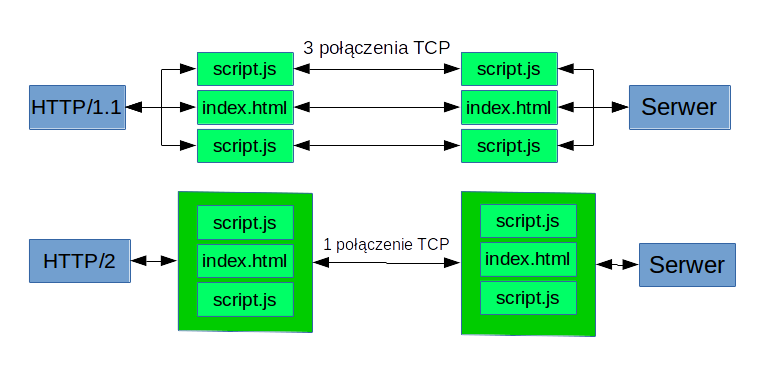
\includegraphics[width=\textwidth]{http2-mux.png}
	\caption{Multipeksowanie HTTP/2}
\end{figure}

\subsection{Proces ładowania strony internetowej i jej zasobów}

Końcowym produktem przeglądarki internetowej jest w pełni załadowana i wyrenderowana strona internetowa, która oferuje użytkownikowi wszystkie zaimplementowane wcześniej funkcjonalności. Proces, który jest odpowiedzialny za dostarczenie tego produktu można podzielić na cztery główne etapy.

\begin{enumerate}
  \item żądanie i odpowiedź
  \item parsowanie
  \item budowanie
  \item renderowanie
\end{enumerate}

\subsubsection{Żądanie i odpowiedź}

Najpopularniejsze przypadki tworzenia nowego żądania przez przeglądarkę internetową są generowane przez użytkownika poprzez:

\begin{enumerate}
  \item wpisanie adresu strony internetowej
  \item kliknięcie na odnośnik przekierowujący do innej strony lub do podstrony aktualnej strony internetowej
  \item przeładowanie aktualnej strony internetowej
\end{enumerate}

Moment tworzenia nowego żadania równoznaczny jest z wydarzeniem które nosi nazwę "\emph{Navigation Start}". Zdarzenie to jest punktem, w którym przeglądarka zaczyna zbierać dodatkowe informacje na temat wydajności np. o czasie ładowania strony. Przeglądarka internetowa tworzy żądanie zgodnie z zasadami protokołu HTTP/1.1, który został bardziej szczegółowo opisny w rozdziale \ref{http/1.1}. Jeśli serwer wspiera obsługę nowszej wersji HTTP/2 wtedy wykorzystany jest nowszy protokół opisany w rozdziale \ref{http/2}. Całe wykonanie żądania przez przeglądarkę możemy podzielić na poszczególne fazy:

\begin{enumerate}
  \item \emph{Kolejkowanie} - przeglądarka kolejkuje żądania w następujących sytuacjach:
    \begin{itemize}
      \item aktualnie istnieją inne żądania do przetworzenia o wyższym priorytecie
      \item aktualnie istnieje już sześć otwartych połączen TCP dla konkretnego źródła (ang. \emph{origin}). Ograniczenie to dotyczy tylko HTTP/1.0 oraz HTTP/1.1
    \end{itemize}
  \item \emph{Odroczenie} - żądanie czeka na swoją kolej na przetworzenie z przyczyn wymienionych we wcześniejszym podpunkcie
  \item \emph{Podgląd DNS} - przeglądarka stara się przetłumaczyć adres internetowy na adres IP za pomocą usługi systemu nazw domenowych (ang. \emph{Domain Name System})
  \item \emph{Negocjowanie z pośrednikiem} - przeglądarka prowadzi negocjacje z serwerem pośredniczącym (ang. \emph{proxy})
  \item \emph{Wysłanie żądania} - przeglądarka wysyła żądanie do serwera
  \item \emph{Oczekiwanie} - przeglądarka oczekuje na pierwsze bajty odpowiedzi, w tym czasie mierzony jest parametr TTFB (ang. \emph{Time To First Byte}) oznaczający czas jaki minął zanim przeglądarka otrzymała pierwszy bajt odpowiedzi
  \item \emph{Pobieranie zawartości} - przeglądarka pobiera całą zawartość odpowiedzi
  \item \emph{Otrzymanie notyfikacji Push} - serwer wysyła dodatkowe dane dla przeglądarki, jest to element unikalny dla HTTP/2
  \item \emph{Czytanie notyfikacji Push} - przeglądarka czyta oraz interpretuje otrzymane wcześniej dodatkowe dane
\end{enumerate}

\begin{figure}[ht]
  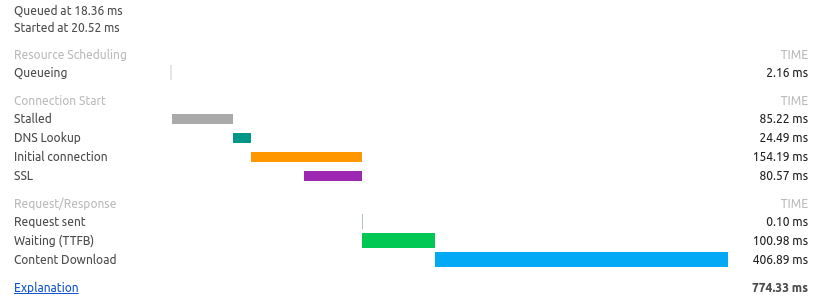
\includegraphics[width=\textwidth]{request-timing-chrome.png}
	\caption{Przykładowy wykres przedstawiający czas trwania poszczególnych faz przetwarzania żądania wygenerowany w przeglądarce Chrome}
\end{figure}

\subsubsection{Parsowanie}

W momencie gdy przeglądarka w pełni przetworzy żądanie i otrzyma dokument w postaci pliku zawierającego kod HTML wtedy następuje proces czytania treści tego pliku w procesie zwanym parsowaniem. Pod pojęciem parsowanie ukrywa się czytanie treści z uwzględnieniem analizy składniowej specyficznej dla konkretnego języka. W przypadku języka HTML przeglądarka oczekuje znaczników z parametrami. 

Jeśli przeglądarka napotka znacznik odnoszący się do kolejnego zasobu wtedy proces parsowania zostaje zatrzymany i tworzone jest żądanie  w celu pobrania zawartości potrzebnej do pełnego wyświetlenia strony. Dopiero gdy przeglądarka pobierze cały zewnętrzny zasób proces parsowania zostaje kontynuowany. Znaczniki blokujące poprzez tworzenie odniesienia do zewnętrznego zasobu to:

\begin{enumerate}
  \item \emph{<link rel="stylesheet" type="text/css" href="style.css\">} - załączenie pliku ze stylami CSS
  \item \emph{<script type="text/javascript\" src="script.js\">} - załączenie pliku z kodem w języku JavaScript
  \item \emph{<img src="image.png\">} - załączenie pliku graficznego
\end{enumerate}

\subsubsection{Budowanie}

W chwili, w której przeglądarka zakończy parsowanie dokumentu i wszystkie zewnętrzne zasoby zostaną pobrane następuje proces budowania strony, czyli łączenia informacji znalezionych w głównym pliku HTML oraz pobranych zasobach. Na budowę strony składają się trzy kroki:

\begin{enumerate}
  \item \emph{Konstrukcja DOM} - obiektowa reprezentacja struktury opisanej w pliku HTML. Szerzej opisana w rozdziale \ref{dom}
  \item \emph{Konstrukcja CSSOM} - obiektowa reprezentacja kaskadowych arkuszy stylów. Szerzej opisana w rozdziale \ref{cssom}
  \item \emph{Konstrukcja Render Tree} - połączenie DOM oraz CSSOM, na podstawie którego przeglądarka jest w stanie poprawnie wyświetlić stronę internetową
\end{enumerate}

\subsubsection{Renderowanie}

Po wykonaniu wszystkich wcześniejszych kroków przeglądarka jest w końcu gotowa aby zacząć wyświetlanie elementów na ekranie. Na ten etap składają się dwa kroki:

\begin{enumerate}
  \item \emph{Layout / Reflow} - przeglądarka wie już co wyświetlić na podstawie DOM, wie też w jaki sposób to wyświetlić na podstawie CSSOM oraz zna relację pomiędzy tymi dwoma elementami na podstawie Render Tree. Rzeczą, której nie wie jest rozmiar elementów, które musi wyświetlić oraz miejsce na ekranie, w którym umieścić poszczególne elementy. Atrybuty takie jak np. szerokość elementów może być ustawiona relatywnie względem rodzica np. 25\% co dodatkowo powoduje problem z wyświetleniem ponieważ potrzebna jest wtedy informacja o wielkości tego rodzica. Ten krok odpowiedzialny jest właśnie za określenie wszystkich tych niewiadomych na podstawie szerokości ekranu (który jest korzeniem w tej strukturze) i wszystkie relatywne wartości bezpośrednich dzieci obliczane są na podstawie niego
  \item \emph{Paint} - po skończeniu wszystkich obliczeń z punktu poprzedniegop rzeglądarka konwertuje każdy węzeł Render Tree na rzeczywiste piksele wyświetlane na ekranie. Użytkownik w pełni widzi oraz może korzystać ze strony internetowej
\end{enumerate}

\subsection{Model współbieżności oraz pętla zdarzeń}

Język JavaScript posiada model współbieżności opary na pętli zdarzeń (ang. \emph{event loop}. Ten model różni się od modeli zaimplementowanych w innych językach jak np. \emph{C} lub \emph{Java}.

Poniższe sekcje wyjaśniają model teoretyczny. Nowoczesne silniki JavaScript implementują i optymalizują opisaną semantykę.

\begin{figure}[ht]
  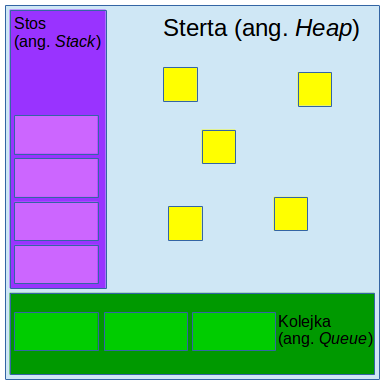
\includegraphics[width=\textwidth]{concurrency-model.png}
	\caption{Wizualizacja modelu}
\end{figure}

\subsubsection{Stos}

Wywołania funkcji tworzą ramki (ang. \emph{frames}), które odkładane są na strukturze danych o nazwie stos(ang. \emph{stack}).

\begin{lstlisting}
function foo(b) {
  var a = 1;
  return a + b;
}

function bar(x) {
  var y = 1;
  return foo(x * y);
}

console.log(bar(2));
\end{lstlisting}

Na przedstawionym przykładzie w momencie wywołania funkcji \emph{bar} zostaje utworzona pierwsza ramka przechowująca argumenty przekazane do tej funkcji oraz lokalne zmienne. Następnie gdy wewnątrz funkcji \emph{bar} wywoływana jest funkcja \emph{foo} tworzona jest druga ramka przechowująca te same informacje tj. przekazane argumenty oraz lokalne zmienne. Ramka umieszczana jest na samej górze stosu nad pierwszym elementem. Kiedy następuje powrót z funkcji \emph{foo} element na samej górze stosu zostaje zdjęty (pozostawijąc tylko ramkę powiązaną z wywołaniem funkcji \emph{bar}). Po powrocie z funkcji \emph{bar} stos powonie staje się pusty.

\subsubsection{Sterta}

Obiekty utworzone w języku JavaScript są umieszczane w stercie (ang. \emph{heap}). Poprzez stertę rozumi się duzą w większości nieustrukturyzowaną przestrzeń pamięci.

\subsubsection{Kolejka}

Środowisko wykonawcze języka JavaScript zawiera kolejkę (ang. \emph{queue}), która składa się z wiadomości do przetworzenia. Funkcja jest przypisana do odpowiedniej wiadomości. W momencie gdy stos posiada wystarczająco dużo miejsca wiadomość jest pobierana z kolejki i przetwarzana. Przetwarzanie polega na wywołaniu skojarzonej funkcji, a tym samym utworzeniu początkowej ramki stosu.
Przetwarzanie wiadomości kończy się, gdy stos staje się pusty.

\subsubsection{Pętla zdarzeń}

Pętla zdarzeń uzyskała swoją nazwę ze względu na to, jak zwykle jest to implementowana. Działanie pętli zdarzen obrazuje poniższy pseudokod:

\begin{lstlisting}
while (queue.waitForMessage()) {
  queue.processNextMessage();
}
\end{lstlisting}

Fragment \emph{queue.waitForMessage()} oczekuje synchronicznie, aż pojawi się wiadomość w kolejkce. Pętla zdarzen posiada kilka bardzo ważnych własności:

\begin{enumerate}
  \item \emph{Działanie do końca} - każda wiadomość jest przetwarzana całkowice przed przetworzeniem jakiejkolwiek innej wiadomości. To zachowanie gwarantuje, iż raz wywołana funkcja będzie działać do końca przed uruchomieniem dowolnego innego kodu. Jako przykład innego działania można przedstawić język C, gdzie np. jeśli funkcja dziąła w wątku może być zatrzymana w dowolnym momencie, aby uruchomić inny kod w innym wątku. Minusem tego modelu jest możliwość zaistnienia sytuacji w której przetwarzanie wiadomości trwa bardzo długo, w tym czasie aplikacja internetowa nie jest w stanie przetworzyć interakcji użytkownika. Przeglądarka obsługuje tą sytuację wyświetlając informację o tym, że wykonywanie skryptu trwa bardzo długo. Może to zniechęcić użytkownika do opuszczenia strony lub jej ponownego odświeżenia. Dobrą praktyką jest pisanie jak najkrótszej implementacji przetwarzania wiadomości
  \item \emph{Sposób dodawania wiadomości} - w przeglądarce internetowej wiadomości dodawane są do kolejki w dowolnym momencie, w którym zdarzenie to ma miejsce pod warunkiem, że została dodana funkcja nasłuchująca konkretnego wydarzenia. Bez nasłuchiwania zdarzenia wiadomość ulega przepadnięciu. Istnieje możliwość dodanie wiadomości do kolejki za pomocą funkcji \emph{setTimeout}. Wiadomość ta zostanie dodana do kolejki po upływie czasu podanego jako argument funkcji. W przypadku, w którym w kolejce nie ma innej wiadomości to nowo dodana wiadomość zostanie przetworzona od razu, jeśli istnieją jakieś inne, wtedy komunikat dodany metodą \emph{setTimeout} będzie musiał poczekać zanim nie zostaną one przetworzone. Z tego powodu argument podany jako czas wkazuje na minimalny czas, a nie na gwarantowany czas. Z tego powodu należy również mieć na uwadze fakt, iż wywołanie funkcji \emph{setTimeout} z opóżnieniem 0 milisekund nie spowoduje przetworzena wiadomości od razu. Wszystko zależy od aktualnego stopnia zapełnienia kolejki.
  \item \emph{Brak blokowania} - w przeciwieńswie do wielu innych języków JavaScript nigdy się nie blokuje. Obsługa wejścia / wyjścia zazwyczaj odbywa się za pośrednictwem zdarzeń i wywołan zwrotnych. Tym samym gdy aplikacja nadal może przetwarzać inne rzeczy jak np. wprowadzanie danych przez użytkownika
\end{enumerate}

\section{Serwer dla aplikacji internetowych} \label{server}

\subsubsection{Opis}

\subsubsection{Implementacja}

\subsubsection{Komponenty}

\section{Biblioteki programistyczne do tworzenia aplikacji internetowyuch}

\subsection{Cechy}

\subsection{Porównanie}

\subsection{Angular 1}

\subsubsection{Opis}

\subsubsection{Wady i zalety}

\subsubsection{Mechanizm działania}

\subsubsection{Implementacja}

\subsection{Angular 2}

\subsubsection{Opis}

\subsubsection{Wady i zalety}

\subsubsection{Mechanizm działania}

\subsubsection{Implementacja}

\subsection{React}

\subsubsection{Opis}

\subsubsection{Wady i zalety}

\subsubsection{Mechanizm działania}

\subsubsection{Implementacja}

\subsection{Vue.js}

\subsubsection{Opis}

\subsubsection{Wady i zalety}

\subsubsection{Mechanizm działania}

\subsubsection{Implementacja}

\subsection{Mithril.js}

\subsubsection{Opis}

\subsubsection{Wady i zalety}

\subsubsection{Mechanizm działania}

\subsubsection{Implementacja}

\section{Badania wydajnościowe}

\subsection{Chrome DevTools}

\cite{chrome-devtools}

\subsection{Badania wydajności pamięciowej}

\subsection{Badania wydajności czasowej}

\section{Porównanie wyników i wnioski}

\section{Podsumowanie}

\subsection{Dalszy rozwój}

\begin{thebibliography}{11}
  \bibitem{milligram}
    \url{http://milligram.io/}
  \bibitem{node.js}
    \url{http://nodejs.org/}
  \bibitem{v8}
    \url{https://github.com/v8/v8}
  \bibitem{npm}
    \url{https://www.npmjs.com/}
  \bibitem{yarn}
    \url{https://yarnpkg.com/}
  \bibitem{es2016}
    \url{https://www.ecma-international.org/ecma-262/7.0/}
  \bibitem{spdy}
    \url{http://dev.chromium.org/spdy/}
  \bibitem{w3c}
    \url{https://www.w3.org/}
  \bibitem{w3c-rec-html51}
    \url{https://www.w3.org/TR/html51/}
  \bibitem{w3c-rec-css3-background}
    \url{https://www.w3.org/TR/css3-background/}
  \bibitem{w3c-rec-css3-box}
    \url{https://www.w3.org/TR/css3-box/}
  \bibitem{w3c-rec-css3-cascade}
    \url{https://www.w3.org/TR/css-cascade-3/}
  \bibitem{w3c-rec-css3-color}
    \url{https://www.w3.org/TR/css3-color/}
  \bibitem{w3c-rec-css3-content}
    \url{https://www.w3.org/TR/css-content-3/}
  \bibitem{w3c-rec-css3-fonts}
    \url{https://www.w3.org/TR/css-fonts-3/}
  \bibitem{w3c-rec-css3-gcpm}
    \url{https://www.w3.org/TR/css-gcpm-3/}
  \bibitem{w3c-rec-css3-template}
    \url{https://www.w3.org/TR/css-template-3/}
  \bibitem{w3c-rec-css3-mediaqueries}
    \url{https://www.w3.org/TR/css3-mediaqueries/}
  \bibitem{w3c-rec-css3-multicol}
    \url{https://www.w3.org/TR/css3-multicol/}
  \bibitem{w3c-rec-css3-page}
    \url{https://www.w3.org/TR/css3-page/}
  \bibitem{w3c-rec-css3-selectors}
    \url{https://www.w3.org/TR/css3-selectors/}
  \bibitem{w3c-rec-css3-ui}
    \url{https://www.w3.org/TR/css-ui-3/}
  \bibitem{w3c-rec-dom-level-1}
    \url{https://www.w3.org/TR/DOM-Level-1/}
  \bibitem{w3c-rec-dom-level-2}
    \url{https://www.w3.org/TR/DOM-Level-2/}
  \bibitem{w3c-rec-dom-level-3-core}
    \url{https://www.w3.org/TR/DOM-Level-3-Core/}
  \bibitem{w3c-rec-dom-level-3-ls}
    \url{https://www.w3.org/TR/DOM-Level-3-LS/}
  \bibitem{w3c-rec-dom-level-3-xpath}
    \url{https://www.w3.org/TR/DOM-Level-3-XPath/}
  \bibitem{w3c-rec-dom-level-3-views}
    \url{https://www.w3.org/TR/DOM-Level-3-Views/}
  \bibitem{w3c-rec-dom-level-3-requirements}
    \url{https://www.w3.org/TR/DOM-Requirements/}
  \bibitem{w3c-rec-dom-level-3-val}
    \url{https://www.w3.org/TR/DOM-Level-3-Val/}
  \bibitem{rfc2616}
    \url{https://www.ietf.org/rfc/rfc2616}
  \bibitem{rfc2660}
    \url{https://www.ietf.org/rfc/rfc2660}
  \bibitem{rfc7540}
    \url{https://www.ietf.org/rfc/rfc7540}
  \bibitem{chrome-devtools}
    \url{https://developers.google.com/web/tools/chrome-devtools/}
\end{thebibliography}

\end{document}
